\newpage
\subsection{QuizziPedia::Front-End::Services}
\begin{figure}
	\centering
	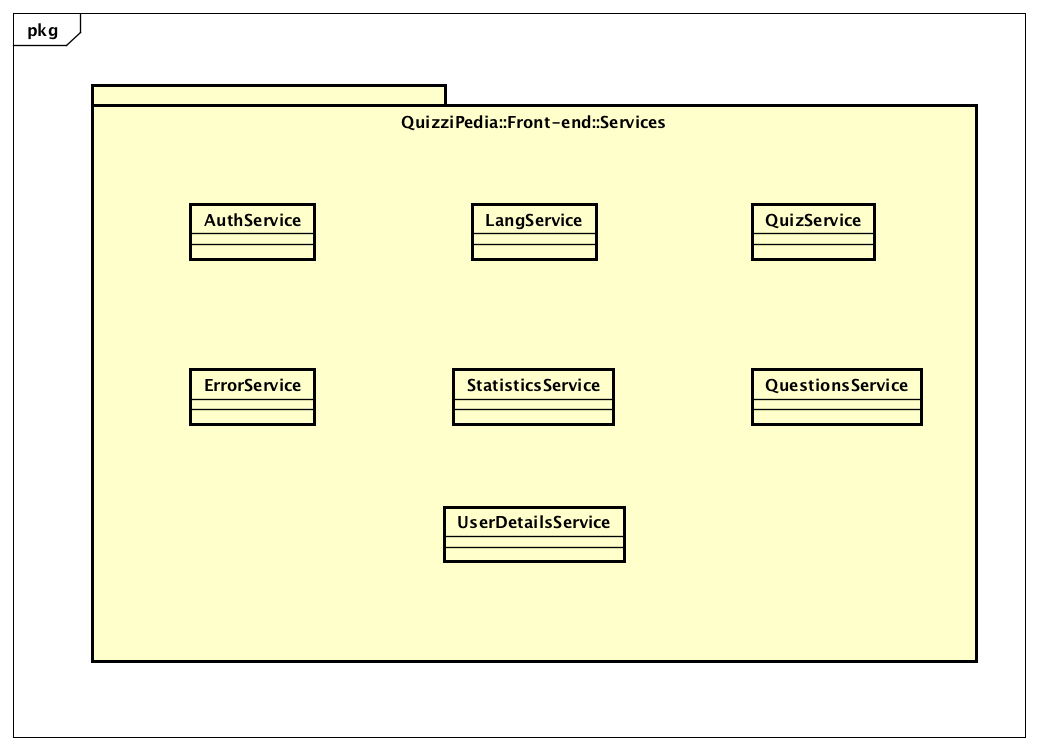
\includegraphics[scale=0.45]{UML/Package/QuizziPedia_Front-End_Services.png}
	\caption{QuizziPedia::Front-End::Services}
\end{figure}
\subsubsection{Informazioni generali}
\begin{itemize}
	\item \textbf{Descrizione}: package che contiene le classi individuate che permettono la comunicazione del lato front-end con il lato back-end;
	\item \textbf{Padre:} \texttt{Front-End};
	\item \textbf{Interazione con altri componenti:}
	\begin{itemize}
		\item \texttt{Models} - package che contiene le classi model individuate;
		\item \texttt{Controllers} - package che contiene le classi controller individuate.
	\end{itemize} 
\end{itemize}
\subsubsection{Classi}

\paragraph{QuizziPedia::Front-End::Services::AuthService}
\begin{figure}
	\centering
	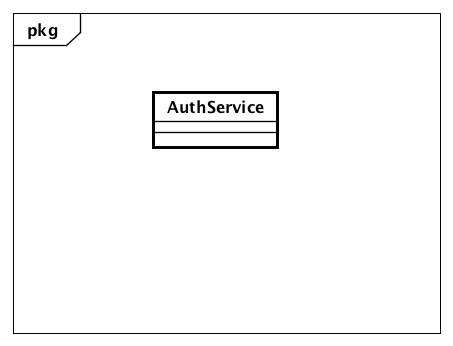
\includegraphics[scale=0.45]{UML/Classi/Front-End/QuizziPedia_Front-end_Services_ AuthService.png}
	\caption{QuizziPedia::Front-End::Services::AuthService}
\end{figure}
\begin{itemize}
	\item \textbf{Descrizione}: questa classe permette di gestire la registrazione e l'autenticazione di un utente;
	\item \textbf{Utilizzo}: fornisce le funzionalità di registrazione e autenticazione ai controllers. Controlla che i dati inseriti dall'utente siano presenti nel \textit{Database\ped{G}} in caso di autenticazione. Presenta anche le funzionalità per la gestione del reset della password;
	\item \textbf{Relazione con altre classi:}
	\begin{itemize}
		\item \textit{IN} \texttt{LoginController}: questa classe gestisce la logica alla base della pagina di autenticazione;
		\item \textit{IN} \texttt{PasswordForgotController}: questa classe gestisce la logica alla base del reset della password;
		\item \textit{IN} \texttt{SignUpController}: questa classe gestisce la logica alla base della registrazione di un nuovo utente.
	\end{itemize}
	\item \textbf{Attributi:}
	\begin{itemize}
		\item 
	\end{itemize}
	\item \textbf{Metodi:}
	\begin{itemize}
		\item 
	\end{itemize}
\end{itemize}

\paragraph{QuizziPedia::Front-End::Services::LangService}
\begin{figure}
	\centering
	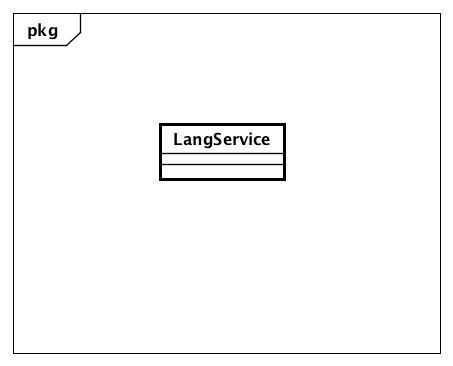
\includegraphics[scale=0.45]{UML/Classi/Front-End/QuizziPedia_Front-end_Services_ LangService.png}
	\caption{QuizziPedia::Front-End::Services::LangService}
\end{figure}
\begin{itemize}
	\item \textbf{Descrizione}: questa classe permette di gestire la lingua nella quale si è scelto di utilizzare l'applicazione.
	\item \textbf{Utilizzo}: fornisce delle funzionalità per recuperare la giusta traduzione della pagina.
	\item \textbf{Relazione con altre classi:}
	\begin{itemize}
		\item \textit{IN} \texttt{LoginController}: questa classe permette di gestire l'autenticazione dell'utente al sistema; 
		\item \textit{IN} \texttt{SignUpController}: questa classe permette di gestire la registrazione di un utente al sistema;
		\item \textit{IN} \texttt{HomeController}: questa classe permette di gestire la home page;
		\item \textit{IN} \texttt{SearchController}: questa classe permette di gestire la ricerca di questionari e utenti all'interno dell'applicazione;
		\item \textit{IN} \texttt{ProfileManagementController}: questa classe permette di gestire il profilo personale di un utente;
		\item \textit{IN} \texttt{LogoutController}: questa classe permette di gestire la pagina di logout;
		\item \textit{IN} \texttt{PasswordForgotController}: questa classe permette di gestire il ripristino della password dimenticata;
		\item \textit{IN} \texttt{TrueFalseController}: questa classe permette di gestire la creazione e la modifica di una domanda vero/falso;
		\item \textit{IN} \texttt{MultiplyQuestionsController}: questa classe permette di gestire la creazione e la modifica di una domanda a risposta multipla; 
		\item \textit{IN} \texttt{ConnectionQuestionsController}: questa classe permette di gestire la creazione e la modifica di una domanda a collegamento;
		\item \textit{IN} \texttt{ImagesSortingQuestionsController}: questa classe permette di gestire la creazione e la modifica di una domanda a ordinamento immagini;
		\item \textit{IN} \texttt{StringsSortingQuestionsController}: questa classe permette di gestire la creazione e la modifica di una domanda a ordinamento di stringhe;
		\item \textit{IN} \texttt{FillingQuestionsController}: questa classe permette di gestire la creazione e la modifica di una domanda a riempimento di spazi; 
		\item \textit{IN} \texttt{ClickableAreaQuestionsController}: questa classe permette di gestire la creazione e la modifica di una domanda ad area cliccabile;
		\item \textit{IN} \texttt{EditorQMLController}: questa classe permette di gestire la creazione e la modifica di domande create tramite editor QML;
		\item \textit{IN} \texttt{QuestionsManagementController}: questa classe permette di gestire e di ottenere le domande create dall'utente;
		\item \textit{IN} \texttt{TrainingController}: questa classe permette di gestire la modalità allenamento sottoponendo all'utente le giuste domande adatte al suo livello;
		\item \textit{IN} \texttt{FillingQuestionnaireController}: questa classe permette di gestire la compilazione del questionario;
		\item \textit{IN} \texttt{TemplateQuestionnaireController}: questa classe permette di gestire la creazione di un questionario; 
		\item \textit{IN} \texttt{RegistrationManagementController}: questa classe permette di gestire le iscrizione degli utenti ai questionari;
		\item \textit{IN} \texttt{ResultsController}: questa classe permette di gestire i risultati della ricerca effettuata dall'utente;
		\item \textit{IN} \texttt{QuestionnaireManagementController}: questa classe permette di gestire tutti i questionari creati da un utente;  
		\item \textit{IN} \texttt{MenuBarController}: questa classe permette di gestire il menù fisso per ogni pagina;
		\item \textit{IN} \texttt{FooterController}: questa classe permette di gestire il footer dell'applicazione;
		\item \textit{IN} \texttt{ErrorController}: questa classe permette di gestire tutti i messaggi di errore da mostrare all'utente.
		
	\end{itemize}
	\item \textbf{Attributi:}
	\begin{itemize}
		\item 
	\end{itemize}
	\item \textbf{Metodi:}
	\begin{itemize}
		\item 
	\end{itemize}
\end{itemize}

\paragraph{QuizziPedia::Front-End::Services::QuizService}
\begin{figure}
	\centering
	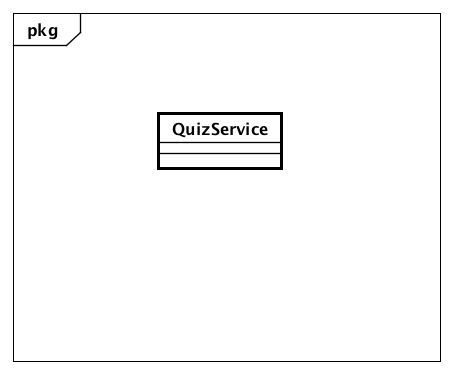
\includegraphics[scale=0.45]{UML/Classi/Front-End/QuizziPedia_Front-end_Services_ QuizService.png}
	\caption{QuizziPedia::Front-End::Services::QuizService}
\end{figure}
\begin{itemize}
	\item \textbf{Descrizione}: questa classe permette di ottenere i dati di un quiz tramite delle parole chiave inserite dall'utente nella barra di ricerca;
	\item \textbf{Utilizzo}: fornisce le funzionalità per ottenere i dati di un quiz in seguito ad una ricerca dell'utente, passando i risultati ai controllers. Ritorna dei riferimenti alle domande del quiz;
	\item \textbf{Relazione con altre classi:}
	\begin{itemize}
		\item \textit{IN} \texttt{SearchController}: questa classe permette di gestire la ricerca di questionari e utenti all'interno dell'applicazione;
		\item \textit{IN} \texttt{QuestionsController}: questa classe permette di gestire il recupero delle domande per poterle stampare nella modalità allenamento;
		\item \textit{IN} \texttt{QuestionnaireDetailsController}: questa classe permette di gestire i dettagli di un questionario;
		\item \textit{IN} \texttt{FillingQuestionnaireController}: questa classe permette di gestire la compilazione del questionario;
		\item \textit{OUT} \texttt{CreateQuestionnaireController}: questa classe permette di gestire la creazione di un questionario;
		\item \textit{OUT} \texttt{RegistrationManagementController}: questa classe permette di gestire le iscrizione degli utenti ai questionari;
		\item \textit{OUT} \texttt{ResultsController}: questa classe permette di gestire le iscrizione degli utenti ai questionari; 
		\item \textit{OUT} \texttt{QuestionnaireManagementController}: questa classe permette di gestire tutti i questionari creati da un utente. 
		
	\end{itemize}
	\item \textbf{Attributi:}
	\begin{itemize}
		\item 
	\end{itemize}
	\item \textbf{Metodi:}
	\begin{itemize}
		\item 
	\end{itemize}
\end{itemize}

\paragraph{QuizziPedia::Front-End::Services::ErrorService}
\begin{figure}
	\centering
	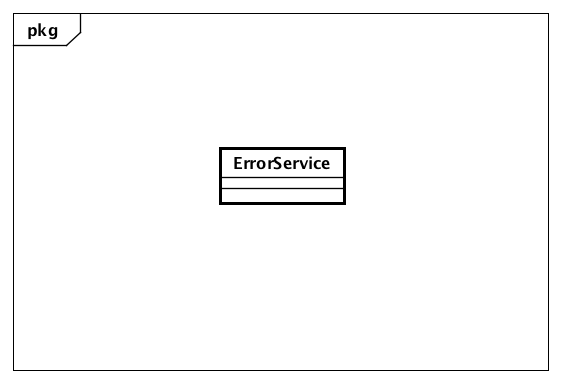
\includegraphics[scale=0.45]{UML/Classi/Front-End/QuizziPedia_Front-end_Services_ ErrorService.png}
	\caption{QuizziPedia::Front-End::Services::ErrorService}
\end{figure}
\begin{itemize}
	\item \textbf{Descrizione}: questa classe permette di gestire il recupero e la gestione dei messaggi di errore;
	\item \textbf{Utilizzo}: fornisce al controller i giusti messaggi di errore da mostrare all'utente;
	\item \textbf{Relazione con altre classi:}
	\begin{itemize}
		\item \textit{IN} \texttt{ErrorController}:questa classe permette di gestire tutti i messaggi di errore da mostrare all'utente. 
	\end{itemize}
	\item \textbf{Attributi:}
	\begin{itemize}
		\item 
	\end{itemize}
	\item \textbf{Metodi:}
	\begin{itemize}
		\item 
	\end{itemize}
\end{itemize}

\paragraph{QuizziPedia::Front-End::Services::StatisticsService}
\begin{figure}
	\centering
	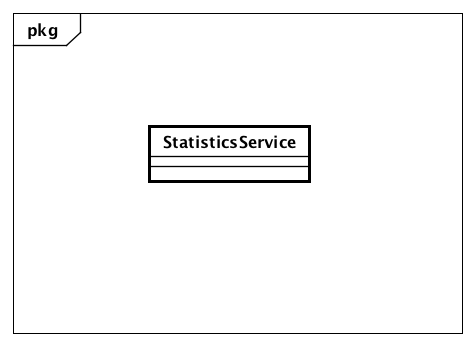
\includegraphics[scale=0.45]{UML/Classi/Front-End/QuizziPedia_Front-end_Services_ StatisticsService.png}
	\caption{QuizziPedia::Front-End::Services::StatisticsService}
\end{figure}
\begin{itemize}
	\item \textbf{Descrizione}: questa classe permette di ottenere le statistiche dell'utente;
	\item \textbf{Utilizzo}: fornisce al controller le statistiche salvate;
	\item \textbf{Relazione con altre classi:}
	\begin{itemize}
		\item \textit{IN} \texttt{StatisticsController}: questa classe permette di le statistiche di un utente.
	\end{itemize}
	\item \textbf{Attributi:}
	\begin{itemize}
		\item 
	\end{itemize}
	\item \textbf{Metodi:}
	\begin{itemize}
		\item 
	\end{itemize}
\end{itemize}

\paragraph{QuizziPedia::Front-End::Services::QuestionServices}
\begin{figure}
	\centering
	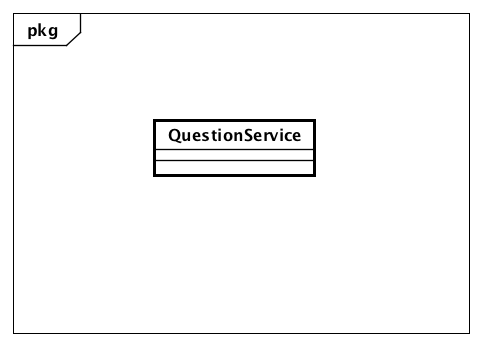
\includegraphics[scale=0.45]{UML/Classi/Front-End/QuizziPedia_Front-end_Services_ QuestionService.png}
	\caption{QuizziPedia::Front-End::Services::QuestionService}
\end{figure}
\begin{itemize}
	\item \textbf{Descrizione}: questa classe permette di ottenere domande esistenti e salvare nuove domande;
	\item \textbf{Utilizzo}: utilizzata per richiedere domande presenti nel database. Offre inoltre delle funzionalità per inserire nuove domande;
	\item \textbf{Relazione con altre classi:}
	\begin{itemize}
		\item \textit{IN} \texttt{TrueFalseController}: questa classe permette di gestire la creazione e la modifica di una domanda vero/falso;
		\item \textit{IN} \texttt{MultiplyQuestionsController}: questa classe permette di gestire la creazione e la modifica di una domanda a risposta multipla; 
		\item \textit{IN} \texttt{ConnectionQuestionsController}: questa classe permette di gestire la creazione e la modifica di una domanda a collegamento;
		\item \textit{IN} \texttt{ImagesSortingQuestionsController}: questa classe permette di gestire la creazione e la modifica di una domanda a ordinamento immagini;
		\item \textit{IN} \texttt{StringsSortingQuestionsController}: questa classe permette di gestire la creazione e la modifica di una domanda a ordinamento di stringhe;
		\item \textit{IN} \texttt{FillingQuestionsController}: questa classe permette di gestire la creazione e la modifica di una domanda a riempimento di spazi; 
		\item \textit{IN} \texttt{ClickableAreaQuestionsController}: questa classe permette di gestire la creazione e la modifica di una domanda ad area cliccabile;
		\item \textit{IN} \texttt{EditorQMLController}: questa classe permette di gestire la creazione e la modifica di domande create tramite editor QML;
		\item \textit{IN} \texttt{QuestionsManagementController}: questa classe permette di gestire e di ottenere le domande create dall'utente
		\item \textit{IN} \texttt{TopicKeywordsController}: questa classe permette di gestire il recupero delle parole chiave di un questionario;
		\item \textit{IN} \texttt{QuestionnaireQuestionsManagementController}: questa classe permette di gestire il recupero delle domande per il questionario.
		
	\end{itemize}
	\item \textbf{Attributi:}
	\begin{itemize}
		\item 
	\end{itemize}
	\item \textbf{Metodi:}
	\begin{itemize}
		\item 
	\end{itemize}
\end{itemize}

\paragraph{QuizziPedia::Front-End::Services::UserDetailsService}
\begin{figure}
	\centering
	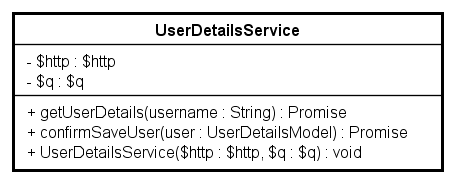
\includegraphics[scale=0.45]{UML/Classi/Front-End/QuizziPedia_Front-end_Services_UserDetailsService.png}
	\caption{QuizziPedia::Front-End::Services::UserDetailsService}
\end{figure}
\begin{itemize}
	\item \textbf{Descrizione}: questa classe permette di ottenere i dati personali degli utenti;
	\item \textbf{Utilizzo}: utilizzata per ottenere i dati personali di un utente. Permette inoltre di trovare i dati di utenti ricercati tramite l'apposita barra di ricerca;
	\item \textbf{Relazione con altre classi:}
	\begin{itemize}
		\item \textit{IN} \texttt{SearchController}: questa classe permette di gestire la ricerca di questionari e utenti all'interno dell'applicazione;
		\item \textit{OUT} \texttt{UserDetailController}: questa classe permette di gestire i dati di un utente;
		\item \textit{OUT} \texttt{ProfileManagementController}: questa classe permette di gestire il profilo personale di un utente. 
	\end{itemize}
	\item \textbf{Attributi:}
	\begin{itemize}
		\item 
	\end{itemize}
	\item \textbf{Metodi:}
	\begin{itemize}
		\item 
	\end{itemize}
\end{itemize}
